\section{Open-XC}\label{apendice:open-xc}
OpenXC es una especificación de hardware y software para ampliar el coche con
aplicaciones y módulos (extensiones por hardware). Mediante un microcontrolador
con firmware de OpenXC instalado, se traducen los mensajes que manda por CAN
el OBD del coche a un formato de mensaje estándar que ha desarrollado OpenXC.

Los vehículos que soportan el estándar son los de marca \"Ford\" puestos
en venta a partir del año 2008. Otras industrias pueden estar implementando el 
estándar, pero no está registrado aún; hay que preguntar por fabricante.

La comunicación desde el interfaz OpenXC hasta el terminal donde se desee ejecutar
la aplicación se realiza a través de una tecnología UART, normalmente se implementa
con bluetooth, ya que es la tecnología de comunicación que mayor flexibilidad ofrece.

\begin{figure}[H]
	\begin{center}
		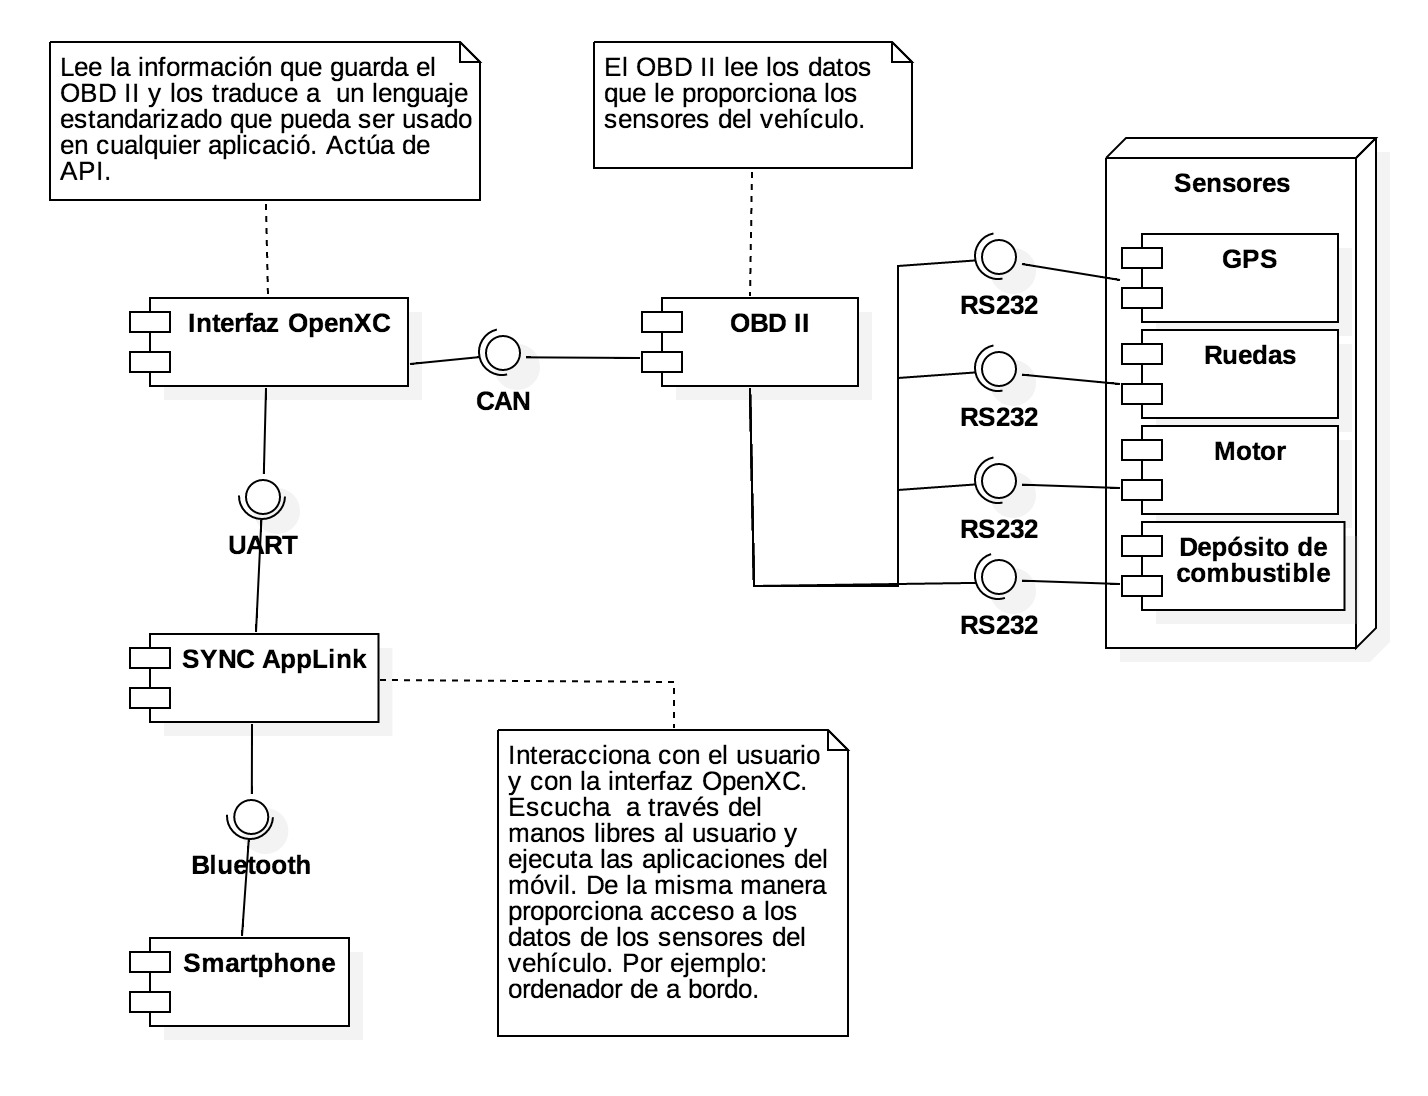
\includegraphics[scale=0.4]{openxc_comunicacion}
		\caption{Comunicación entre componentes en un vehículo con OpenXC instalado.}
		\label{fig:openxc_comunicacion}
	\end{center}
\end{figure}


En la figura \ref{fig:openxc_comunicacion}, se expone una posible implementación del sistema
completo. OBD es el sistema que obtiene los datos de sensores que se encuentran integrados en
los vehículos, a través de un dispositivo móvil por un conector tipo CAN, es posible leer la
información obtenida por el OBD. En este punto es donde entra el Interfaz OpenXC, el cual está
conectado al OBD y traduce los datos obtenidos a un lenguaje estándar para todos los vehículos;
es decir, actúa como un API del vehículo. Al interfaz OpenXC podemos conectar un dispositivo
con Android para ejecutar una aplicación que utilice los métodos que nos ofrece el API de
OpenXC para su funcionamiento. ¿Por qué es necesario el interfaz OpenXC en vez de leer los
datos del OBD? Porque cada vehículo es diferente y no existe un estándar para obtener los datos
de los sensores. Cada OBD II transmite los datos de forma diferente, habría que desarrollar
miles de aplicaciones para todos los coches. La interfaz reconoce el OBD II al que está
conectado y proporciona acceso a los datos, de forma que una aplicación no tiene que cambiar
de coche en coche, ya que de la tarea de traducción es delegada al Interfaz OpenXC.

En una capa superior es posible conectar un dispositivo compatible con el interfaz: Ford, por
ejemplo, conecta su sistema SYNC AppLink el cual hace de intermediario entre el usuario y
vehículo. Lo podríamos identificar como “el ordenador de a bordo”, la parte del Software
y hardware que se muestra al usuario. En Ford, mediante SYNC AppLink se escucha al usuario
a través del manos libres y ejecuta los comandos en el móvil del usuario, previamente
conectado a través de Bluetooth. En el móvil del usuario se guardarán y ejecutarán las
aplicaciones. La comunicación al ser bidireccional permite al usuario ver lo que pasa, por
ejemplo, en una pantalla situada en el cristal delantero.

Otra de las iniciativas que se ofrecen desde OpenXC es hacer que el vehículo no se quede atrás
respecto a la tecnología; por ejemplo, si se adquiere un coche que tiene integrado 2G y en unos
meses sale una tecnología mayor, es imposible cambiarla ya que se encuentra integrada en
el vehículo. Sin embargo, con el interfaz OpenXC es posible habilitar un puerto USB para
introducir un adaptador de 3G, o bluetooth... De esta forma en vez de tener que cambiar una
gran parte del hardware instalado en el coche, tan solo hay que cambiar un adaptador.

\subsection{Recursos necesarios}
Para poder realizar pruebas, en un escenario básico, con esta tecnología es necesario:

\begin{itemize}
	\item Un terminal donde se pueda ejecutar aplicaciones Android, iOS o Python.

	\item Un interfaz OpenXC: leerá los datos de cualquier OBD II y los traducirá en un
	 lenguaje universal para poder ser usado en diferentes plataformas. El precio medio
	 de un interfaz OpenXC es de unos 150\$, existen módulos para compra directa o se
	 puede construir uno, ya que el firmware está disponible públicamente.

	\item API del interfaz OpenXC para el desarrollo de aplicaciones.
	
	\item Un OBD-II.
\end{itemize}